\documentclass[letterpaper,10pt]{article}

\usepackage{titling}
\usepackage{listings}
\usepackage{url}
\usepackage{setspace}
\usepackage{subfig}
\usepackage{sectsty}
\usepackage{pdfpages}
\usepackage{colortbl}
\usepackage{multirow}
\usepackage{multicol}
\usepackage{relsize}
\usepackage{amsmath}
\usepackage{fancyvrb}
\usepackage[yyyymmdd]{datetime}
\usepackage{amsmath,amssymb,amsthm,graphicx,xspace}
\usepackage[titlenotnumbered,noend,noline]{algorithm2e}
\usepackage[compact]{titlesec}
\usepackage{XCharter}
\usepackage[T1]{fontenc}
\usepackage{tikz}
\usetikzlibrary{arrows,automata,shapes,trees,matrix,chains,scopes,positioning,calc}
\tikzstyle{block} = [rectangle, draw, fill=blue!20, 
    text width=2.5em, text centered, rounded corners, minimum height=2em]
\tikzstyle{bw} = [rectangle, draw, fill=blue!20, 
    text width=4em, text centered, rounded corners, minimum height=2em]

\definecolor{namerow}{cmyk}{.40,.40,.40,.40}
\definecolor{namecol}{cmyk}{.40,.40,.40,.40}
\renewcommand{\dateseparator}{-}


\let\LaTeXtitle\title
\renewcommand{\title}[1]{\LaTeXtitle{\textsf{#1}}}


\newcommand{\handout}[5]{
  \noindent
  \begin{center}
  \framebox{
    \vbox{
      \hbox to 5.78in { {\bf ECE252: Systems Programming and Concurrency } \hfill #2 }
      \vspace{4mm}
      \hbox to 5.78in { {\Large \hfill #4  \hfill} }
      \vspace{2mm}
      \hbox to 5.78in { {\em #3 \hfill \today } }
    }
  }
  \end{center}
  \vspace*{4mm}
}

\newcommand{\lecture}[3]{\handout{#1}{#2}{#3}{Lecture #1}}{
\newcommand{\tuple}[1]{\ensuremath{\left\langle #1 \right\rangle}\xspace}

\addtolength{\oddsidemargin}{-1.000in}
\addtolength{\evensidemargin}{-0.500in}
\addtolength{\textwidth}{2.0in}
\addtolength{\topmargin}{-1.000in}
\addtolength{\textheight}{1.75in}
\addtolength{\parskip}{\baselineskip}
\setlength{\parindent}{0in}
\renewcommand{\baselinestretch}{1.5}
\newcommand{\term}{Spring 2019}

\singlespace


\begin{document}

\lecture{ 11 --- Threads }{\term}{Jeff Zarnett}

\section*{Threads}

Not very long ago we discussed what makes a process. A process has three major components: an executable program, the data created or needed by the program, and the execution context of the program (files opened, resources allocated, et cetera). A process has at least one \textit{thread}, and can have many.

The term ``thread'' is a short form of \textit{Thread of Execution}. A thread of execution is a sequence of executable commands that can be scheduled to run on the CPU. Threads also have some state (where in the sequence of executable commands the program is) and some local variables. Most programs you have written until now probably had only one thread; that is, your program's code is executed one statement at a time, sequentially in some order.

A multithreaded program is one that uses more than one thread, at least some of the time. When a program is started, it begins with an initial thread (where the \texttt{main} function is) and that main thread can create some additional threads if needed. Note that threads can be created and destroyed within a program dynamically: a thread can be created to handle a specific background task, like writing changes to the database, and will terminate when it is done. Or a created thread might be persistent.

In a process that has multiple threads, each thread has its own~\cite{osi}:
\begin{enumerate}
	\item Thread execution state (like process state: running, ready, blocked...).
	\item Saved thread context when not running.
	\item Execution stack.
	\item Local variables.
	\item Access to the memory and resources of the process (shared with all threads in that process).
\end{enumerate}

Or, to represent this visually:

\begin{center}
	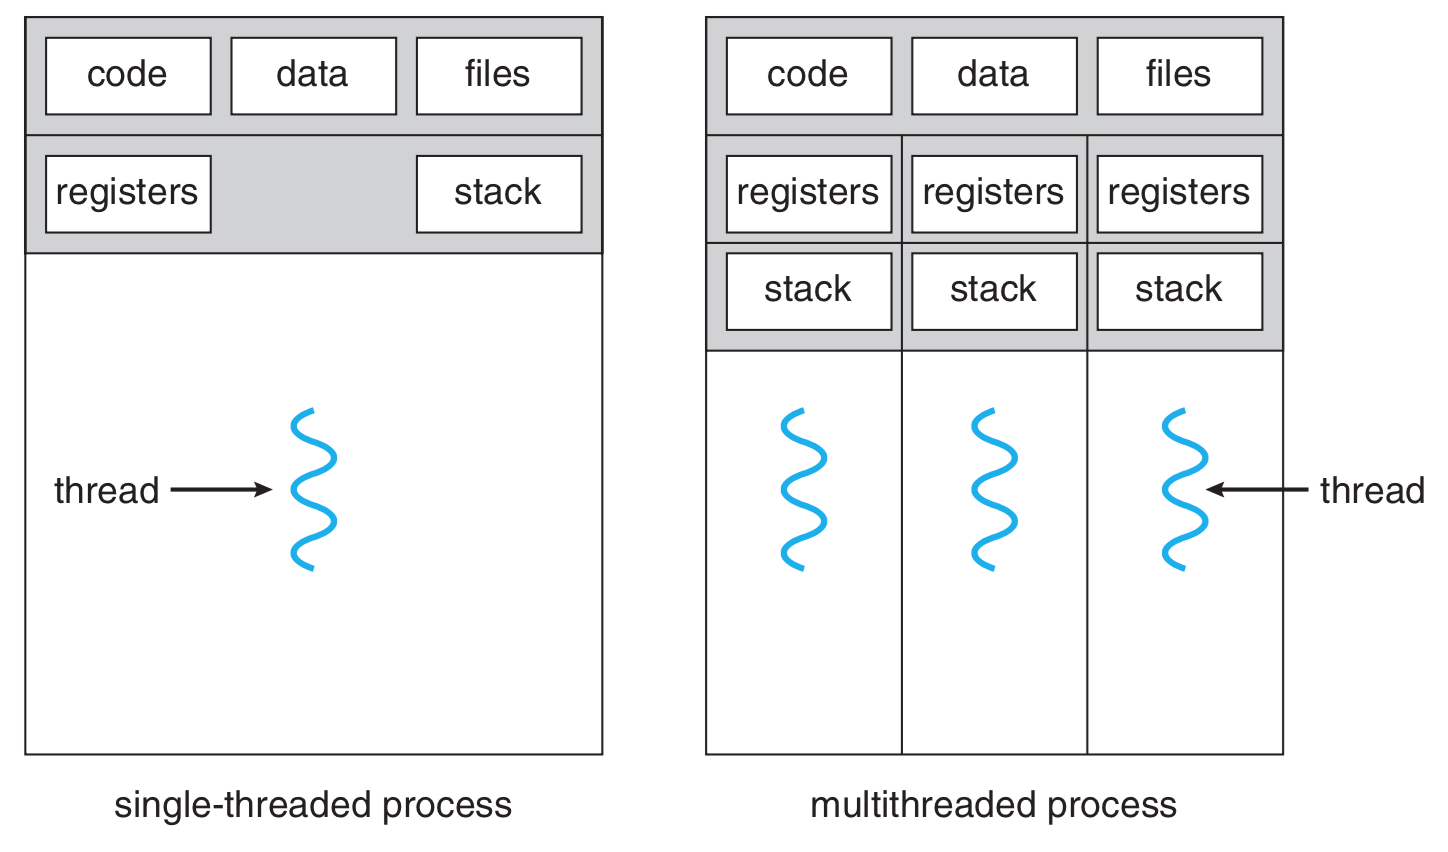
\includegraphics[width=0.625\textwidth]{images/mthread2.png}\\
	A single threaded and a multithreaded process compared side-by-side~\cite{osc}.
\end{center}

All the threads of a process share the state and resources of the process. If one thread opens a file, other threads in that process can also access that file.

The way programs are written now, there are few if any that are not in some way multithreaded. One common way of dividing up the program into threads is to separate the user interface from a time-consuming action. Consider a file-transfer program. If the user interface and upload function share a thread, once a file upload has started, the user will not be able to use the UI anymore (and Windows will put the dreaded ``(Not Responding)'' at the end of its dialog title), even to click the button that cancels the upload. For some reason, users hate that.

We have two options for how to alleviate this problem: when an upload is ready to start, we can call \texttt{fork} and create a new process to do the upload, or we can spawn  new thread. In either case, the newly created entity will handle the upload of the file. The UI remains responsive, because the UI thread is not waiting for the upload function to complete.

\subsection*{Motivation for Threads}

Why choose threads rather than creating a new process? The primary, but not sole, motivation is performance:
\begin{enumerate}
	\item Creating a new thread is much faster than creating a new process. In fact, thread creation is on the order of ten times faster~\cite{machThreads}.
	\item Terminating and cleaning up a thread is faster than terminating and cleaning up a process.
	\item It takes less time to switch between two threads within the same process (because less data needs to be stored/restored). In Solaris, for example, switching between processes is about five times slower than switching between threads~\cite{osc}.
	\item Because threads share the same memory space, for two threads to communicate, they do not have to use any of the IPC mechanisms; they can just communicate directly. This is a bigger item than it might seem like, because inter-task communication can be very expensive.
	\item As in the file transfer program, use of threads allows the program to be responsive even when a part of the program is blocked.
\end{enumerate}

This last advantage, background work, is one of four common examples of the uses of threads in a general purpose operating system~\cite{insideOS2}:
\begin{enumerate}
	\item \textbf{Foreground and Background Work:} as already examined, the ability to run something in the background to keep the program responsive.
	\item \textbf{Asynchronous processing}: for example, to protect against power failure or a crash, a word processor may write the document data in main memory to disk periodically. This can be done as a background task so it does not disrupt the user's workflow. You've probably experienced this in Microsoft Word, for example, if a document is ``recovered''.
	\item \textbf{Speed of Execution:} a multithreaded program can get more done in the same amount of time. Just as the OS can run a different program when the executing program gets blocked (say, on a disk read), if one thread is blocked, another thread may execute. But also, we probably have a computer with many cores, so we can put them all to use.
	\item \textbf{Modular Structure:} a program that does several different things may be given structure through threads. Threads have specific ``jobs'' and they each step in and do their job when it is appropriate for them to do so.
\end{enumerate}

There are some drawbacks, however: there is no protection between threads in the same process: so one thread can easily mess with the memory being used by another thread. This once again brings us to the subject of co-ordination, which will follow the discussion of threads.

Also, if any thread encounters an error (such as a division by zero or Segmentation Fault), the whole process might be terminated by the operating system. If the program has multiple processes for different parts, then the other processes will not be affected; if the program has multiple threads and they all share the same process, then any thread encountering an error might bring all of them to a halt.


\subsection*{Thread States}
Each individual thread will have its own state. We said earlier that a process may have seven states, but the model for thread state will be the somewhat simpler five-state model. If a process is swapped out of memory, all its threads will be swapped out; when that process is swapped in to memory, all the threads will be swapped in. Therefore we do not need to consider whether a thread is in memory or swapped; hence the five-state model, reproduced once again below:

\begin{center}
	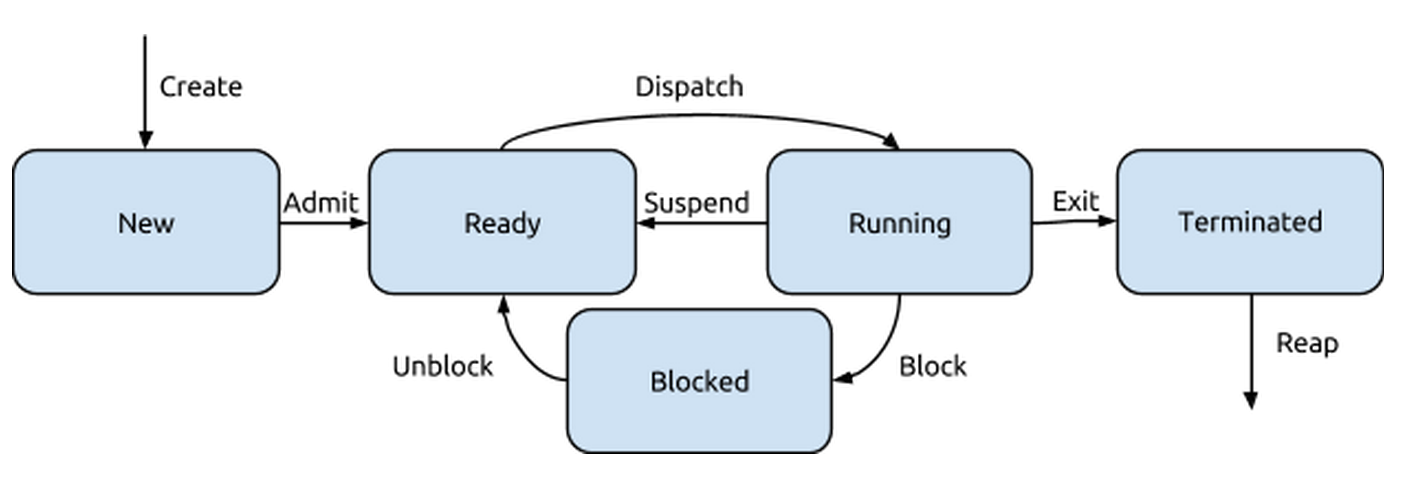
\includegraphics[width=0.85\textwidth]{images/5-state-model.png}\\
	State diagram for the five-state model.
\end{center}

The transitions work the same way as the state transitions for a process. As with a process, a thread in any state can transition to terminated even though that is not shown on the diagram. When a process is terminated, all its threads are terminated, regardless of what state it is in. The example we started with, the file transfer upload being cancelled, is an example of termination we should consider: thread cancellation.


\section*{POSIX Threads}

The term \texttt{pthread} refers to the POSIX standard (also known as the IEEE 1003.1c standard) that defines thread behaviour in UNIX and UNIX-like systems (Linux, Mac OS X, Solaris...). This is a specification document that says how threads should behave. This standard lets code for one UNIX-like system (e.g., Solaris) run easily on another (e.g., Linux). The POSIX standard for pthreads defines something like 100 function calls, but we need not examine all of them. Let us focus on a few of the important ones and we can see they have some similarity to what we saw with parent and child processes~\cite{mos}:

\begin{itemize}
	\item \texttt{pthread\_create} -- Create a new thread. This works a lot like \texttt{fork}.
	\item \texttt{pthread\_exit} -- Terminate the calling thread. This is like \texttt{exit} in that it ends execution and returns a value.
	\item \texttt{pthread\_join} -- Wait for a specific thread to exit. This is like \texttt{wait}: the caller cannot proceed until the thread it is waiting for calls \texttt{pthread\_exit}. Note that it is an error to join a thread that has already been joined.
	\item \texttt{pthread\_detach} -- If we want to make it so that a thread cannot be joined, then we can make it a ``detached'' thread with this function.
	\item \texttt{pthread\_yield} -- Release the CPU and let another thread run. As they all belong to the same program, we expect that threads want to co-operate rather then compete for CPU time and threads can make decisions about when it would be ideal to let some other thread run instead.
	\item \texttt{pthread\_attr\_init} -- Create and initialize a thread's attributes. The attributes contain things like the priority of the thread. (``After you, sir.'' ``Oh no, after you.'')
	\item \texttt{pthread\_attr\_destroy} -- Remove a thread's attributes. Free up the memory holding the thread's attributes. This does not terminate the threads.
	\item \texttt{pthread\_cancel} -- Signal cancellation to a thread; this can be asynchronous or deferred, depending on the thread's attributes.
	\item \texttt{pthread\_testcancel} -- A thread can check to see if it has been cancelled. If that is the case, this function terminates the calling thread.
\end{itemize}

This list of functions gives us an overview of the toolkit we have, but we need to elaborate with some examples to fully understand how they work.

\paragraph{Creating a New Thread.}

When we want to start a new thread, we have to say what that new thread is supposed to do. The function signature for \texttt{pthread\_create} looks like:

\begin{lstlisting}[language=C]
pthread_create( pthread_t *thread, const pthread_attr_t * attr, void *(*start_routine)( void * ), void *arg );
\end{lstlisting}

Where: \texttt{thread} is a pointer to a \texttt{pthread} identifier and will be assigned a value when the thread is created. The attributes \texttt{attr} may contain various characteristics (but you may supply \texttt{NULL} if you want the defaults). The third parameter is the function to run, but it requires a little more explanation.The last parameter, \texttt{arguments} is the argument passed to the \texttt{start\_routine}. But that second last one is weird.

The \texttt{start\_routine} parameter is the name of any function that takes a single untyped pointer and returns an untyped pointer. That is, the function signature has to match those two conditions. The name of the function (and the name of the argument) can be anything you like. See the example below:

\begin{lstlisting}[language=C]
void* do_something( void* start_params )
\end{lstlisting}


After the new thread has been created, the process has two threads in it. The OS makes no guarantee about which thread will be executing after the new one is created; this is a matter of scheduling. It could be either of the threads of the process, both of them at the same time, or a different process entirely.

Our experience with C-like languages suggests it is normal to have a single return value from a function, but usually we can have multiple input parameters. It seems limiting to be able to put in just one. There are two ways to get around this: with an array or with structures. In the case of the array, the argument provided to \texttt{pthread\_create} is just a pointer to the array. This is also, incidentally, how you can get multiple return values out of a function in Java or C\# (\texttt{public Object[] foo()}), but I don't recommend it as a good programming practice. The other way to do it is to use the \texttt{struct}, defining a structure for the parameter type and one for the return type.

The function that is to run in the new thread must expect a pointer to the arguments and then it will need to be cast to the appropriate (actual) type:
\begin{lstlisting}[language=C]
void* function( void * void_arg ) {
  parameters_t *arguments = (parameters_t*) args;
  /* continue after this */
}
\end{lstlisting}

This does imply that the caller of the \texttt{pthread\_create} function has to know what kind of argument is expected in the function being called. That is fairly normal; we do have to know what the arguments mean when we pass them in to any function, but in this case we don't have the ``hints'' that the types provide.

What about the thread attributes? They can be used to set whether a thread is detached or joinable, scheduling policy, etc. By default, new threads are usually joinable (that is to say, that some other thread can call \texttt{pthread\_join} on them). As noted before, it is a logical error to attempt multiple joins on the same thread. To prevent a thread from ever being joined, it can be created in the detached state (or the method \texttt{pthread\_detach} can be called on a joinable thread). Trying to join a detached thread is also a logical error~\cite{pthreads}. For virtually all scenarios that we will consider in this course the default values will be fine.

Once we do that, the new thread we created is running. It does whatever its code does, so everything proceeds as expected, until of course the thread gets to the end. Usually, it will terminate with \texttt{pthread\_exit}. The use of \texttt{pthread\_exit} is not the only way that a thread may be terminated. Sometimes we want the thread to persist (hang around), but if we want to get a return value from the thread, then we need it to exit.

\paragraph{Returning Values.} If a thread has no return values, it can just \texttt{return NULL;} which will have the same effect as \texttt{pthread\_exit} and send \texttt{NULL} back to the thread that has joined it. If the function that is called as a task returns normally rather than calling the exit routine, the thread will still be terminated.

Another way a thread might terminate is if the \texttt{pthread\_cancel} function is called with it as the target. As before, if the termination is deferred rather than asynchronous, the thread is responsible for cleaning up after itself before it stops.

A thread may also be terminated indirectly: if the entire process is terminated or if \texttt{main} finishes first (without calling \texttt{pthread\_exit} itself). Indeed, \texttt{main} can use \texttt{pthread\_exit} as the last thing that it does. Without that, \texttt{main} will not wait for other, unjoined threads to finish and they will all get suddenly terminated. If \texttt{main} calls \texttt{pthread\_exit} then it will be blocked until the threads it has spawned have finished~\cite{pthreads}.

\paragraph{Collecting Returned Values.} Like the \texttt{wait} system call, the \texttt{pthread\_join} is how we get a value out of the spawned thread:

\begin{lstlisting}[language=C]
pthread_join( pthread_t thread, void** retval );
\end{lstlisting}

The first parameter specifies the thread that you want to join. The second parameter is... wait... two stars? What we are looking for is a pointer to a void pointer. That is, we are going to supply a pointer that the join function will update to be pointing to the value returned by that function. Typically we supply the address of a pointer. This will be hopefully clearer in the example:

\begin{lstlisting}[language=C]
#include <stdlib.h>
#include <stdio.h>
#include <pthread.h>

void * run( void * argument ) { 
  char* a = (char*) argument;
  printf("Provided argument is %s!\n", a); 
  int * return_val = malloc( sizeof( int )); 
  *return_val = 99; 
  pthread_exit( return_val );
}

int main( int argc, char** argv ) { 
  if (argc != 2) {
      printf("Invalid args.\n");
      return -1; 
  }
  pthread_t t;
  void* vr; 
  
  pthread_create( &t, NULL, run, argv[1] );
  pthread_join( t, &vr );
  int* r = (int*) vr; 
  printf("The other thread returned %d.\n", *r);
  free( vr );
  pthread_exit( 0 );
}
\end{lstlisting}

\bibliographystyle{alphaurl}
\bibliography{252}


\end{document}